%%%%%%%%%%%%%%%%%%%%%%%%%%%%%%%%%%%%%%%%%
% Beamer Presentation
% LaTeX Template
% Version 1.0 (10/11/12)
%
% This template has been downloaded from:
% http://www.LaTeXTemplates.com
%
% License:
% CC BY-NC-SA 3.0 (http://creativecommons.org/licenses/by-nc-sa/3.0/)
%
%%%%%%%%%%%%%%%%%%%%%%%%%%%%%%%%%%%%%%%%%

%----------------------------------------------------------------------------------------
%	PACKAGES AND THEMES
%----------------------------------------------------------------------------------------

%\documentclass[UTF8,aspectratio=169,14pt]{ctexbeamer}
\documentclass[UTF8,aspectratio=169]{ctexbeamer}
\usepackage{hyperref}
\hypersetup{
	colorlinks=true,
	linkcolor=red,
	anchorcolor=blue,
	citecolor=green
}

\mode<presentation> {
	
	% The Beamer class comes with a number of default slide themes
	% which change the colors and layouts of slides. Below this is a list
	% of all the themes, uncomment each in turn to see what they look like.
	
	%\usetheme{default}
	%\usetheme{AnnArbor}
	%\usetheme{Antibes}
	%\usetheme{Bergen}
	%\usetheme{Berkeley}
	%\usetheme{Berlin}
	%\usetheme{Boadilla}
	%\usetheme{CambridgeUS}
	%\usetheme{Copenhagen}
	%\usetheme{Darmstadt}
	%\usetheme{Dresden}
	%\usetheme{Frankfurt}
	%\usetheme{Goettingen}
	%\usetheme{Hannover}
	%\usetheme{Ilmenau}
	%\usetheme{JuanLesPins}
	%\usetheme{Luebeck}
	\usetheme{Madrid}
	%\usetheme{Malmoe}
	%\usetheme{Marburg}
	%\usetheme{Montpellier}
	%\usetheme{PaloAlto}
	%\usetheme{Pittsburgh}
	%\usetheme{Rochester}
	%\usetheme{Singapore}
	%\usetheme{Szeged}
	%\usetheme{Warsaw}
	
	% As well as themes, the Beamer class has a number of color themes
	% for any slide theme. Uncomment each of these in turn to see how it
	% changes the colors of your current slide theme.
	
	%\usecolortheme{albatross}
	%\usecolortheme{beaver}
	%\usecolortheme{beetle}
	%\usecolortheme{crane}
	%\usecolortheme{dolphin}
	%\usecolortheme{dove}
	%\usecolortheme{fly}
	%\usecolortheme{lily}
	%\usecolortheme{orchid}
	%\usecolortheme{rose}
	%\usecolortheme{seagull}
	%\usecolortheme{seahorse}
	%\usecolortheme{whale}
	%\usecolortheme{wolverine}
	
	%\setbeamertemplate{footline} % To remove the footer line in all slides uncomment this line
	%\setbeamertemplate{footline}[page number] % To replace the footer line in all slides with a simple slide count uncomment this line
	
	%\setbeamertemplate{navigation symbols}{} % To remove the navigation symbols from the bottom of all slides uncomment this line
}

\usepackage{graphicx} % Allows including images
\graphicspath{{./figs/}}
\usepackage{booktabs} % Allows the use of \toprule, \midrule and \bottomrule in tables
\usepackage{longtable}
\usepackage{listings}
\usepackage{xcolor}
\lstset{numbers=left, %设置行号位置
	numberstyle=\tiny, %设置行号大小
	keywordstyle=\color{blue}, %设置关键字颜色
	commentstyle=\color[cmyk]{1,0,1,0}, %设置注释颜色
	frame=single, %设置边框格式
	escapeinside=``, %逃逸字符(1左面的键),用于显示中文
	%breaklines, %自动折行
	extendedchars=false, %解决代码跨页时,章节标题,页眉等汉字不显示的问题
	xleftmargin=2em,xrightmargin=2em, aboveskip=1em, %设置边距
	tabsize=4, %设置tab空格数
	showspaces=false %不显示空格
}
% Fonts
% \usepackage{libertine}
% \setmonofont{Courier}
\setCJKsansfont[ItalicFont=Noto Serif CJK SC Black, BoldFont=Noto Sans CJK SC Black]{Noto Sans CJK SC}
\setmainfont[Ligatures={Common,TeX}]{Linux  Libertine O}
\setmonofont[SmallCapsFont={Latin Modern Mono Caps}]{Latin Modern Mono Light}
\setsansfont{Linux Biolinum O}

\logo{
\includegraphics[width=0.55cm,height=0.55cm]{../../thcs-logo.png}}

%----------------------------------------------------------------------------------------
%	TITLE PAGE
%----------------------------------------------------------------------------------------

\title[第6讲]{第6讲 :The Programming Languages of OS} % The short title appears at the bottom of every slide, the full title is only on the title page
\subtitle{第一节:Introduction }
\author{陈渝} % Your name
\institute[清华大学] % Your institution as it will appear on the bottom of every slide, may be shorthand to save space
{
	清华大学计算机系 \\ % Your institution for the title page
	\medskip
	\textit{yuchen@tsinghua.edu.cn} % Your email address
}
\date{\today} % Date, can be changed to a custom date


\begin{document}

\begin{frame}
\titlepage % Print the title page as the first slide
\end{frame}

%\begin{frame}
%\frametitle{提纲} % Table of contents slide, comment this block out to remove it
%\tableofcontents % Throughout your presentation, if you choose to use \section{} and \subsection{} commands, these will automatically be printed on this slide as an overview of your presentation
%\end{frame}
%
%%----------------------------------------------------------------------------------------
%%	PRESENTATION SLIDES
%%----------------------------------------------------------------------------------------
%
%%------------------------------------------------
%\section{第一节:课程概述} % Sections can be created in order to organize your presentation into discrete blocks, all sections and subsections are automatically printed in the table of contents as an overview of the talk
%%------------------------------------------------
%-------------------------------------------------
\begin{frame}[plain]
	\frametitle{Introduction}
	
	
	
	\begin{columns}
		
		\begin{column}{.3\textwidth}
			
			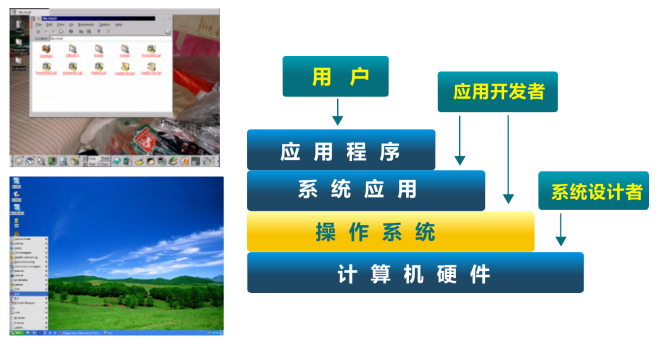
\includegraphics[width=1.\textwidth]{os-position}
			
		\end{column}
		
		\begin{column}{.7\textwidth}
			
			\Large
			Some questions
			\begin{itemize}
				\item  Is Programming Language important for OS?
				\item Is C  the best language for OS?
				\item Which parts of language affect OS deeply?
				\item Other than languages, Which components affect the development of OS? 
				\item Why do we need/needn't to change the language for OS?				
			\end{itemize}
			
		\end{column}
		
		
	\end{columns}
	
	
\end{frame}

%-------------------------------------------------
\begin{frame}[plain]
	\frametitle{Introduction}
	
	
	
	\begin{columns}
		
		\begin{column}{.4\textwidth}
			
			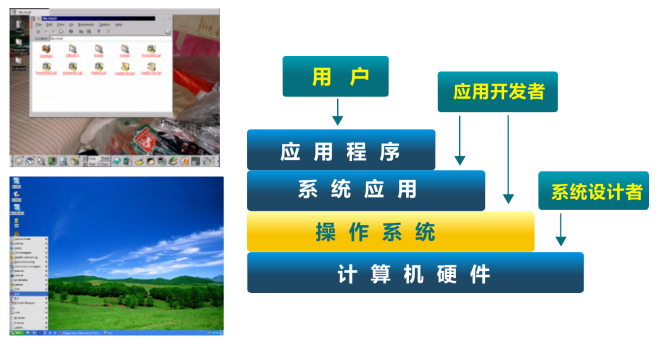
\includegraphics[width=1.\textwidth]{os-position}
			
		\end{column}
		
		\begin{column}{.6\textwidth}
			
	\begin{block}{What is OS}
	An operating system (OS) is system software that manages computer hardware, software resources, and provides common services for computer programs. [wikipedia]
    \end{block} 
	\LARGE
	What is the Programming Languages?

		\end{column}
		
		
	\end{columns}
	
	
\end{frame}


%-------------------------------------------------
\begin{frame}[plain]
	\frametitle{Introduction}
	
	
	
	\begin{columns}
		
		\begin{column}{.4\textwidth}
			
			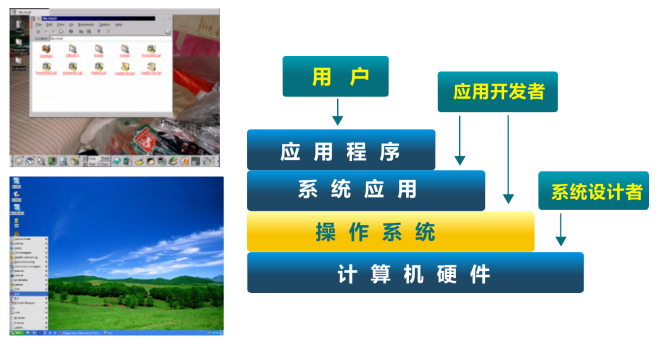
\includegraphics[width=1.\textwidth]{os-position}
			
		\end{column}
		
		\begin{column}{.6\textwidth}
			
			\begin{block}{What is Programming Languages}
				A programming language is a formal language, which comprises a set of instructions that produce various kinds of output. Programming languages are used in computer programming to implement algorithms. [wikipedia]
			\end{block} 
			\LARGE
			What is the Programming Languages for OS?
			
		\end{column}
		
		
	\end{columns}
	
	
\end{frame}


%-------------------------------------------------
\begin{frame}[plain]
	\frametitle{Introduction}

\centering
TIOBE Index for August 2019
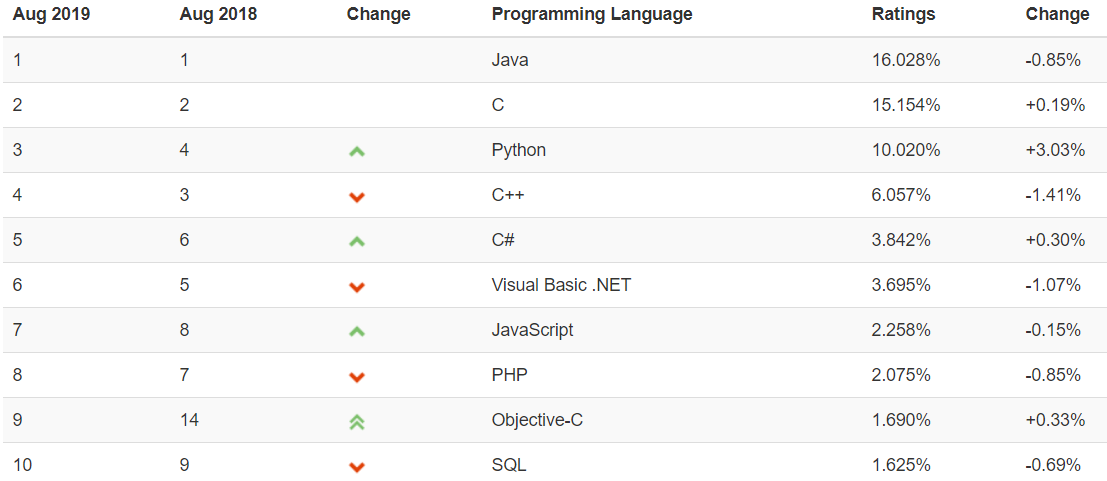
\includegraphics[width=1.\textwidth]{pl-index}
\end{frame}
%-------------------------------------------------


%-------------------------------------------------
\begin{frame}[plain]
	\frametitle{Introduction}
	
	
	
	\begin{columns}
		
		\begin{column}{.4\textwidth}
			
			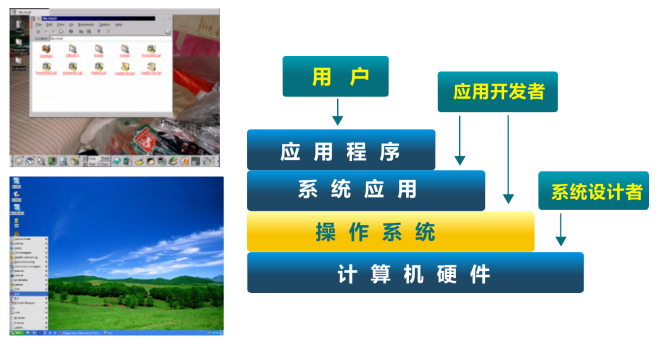
\includegraphics[width=1.\textwidth]{os-position}
			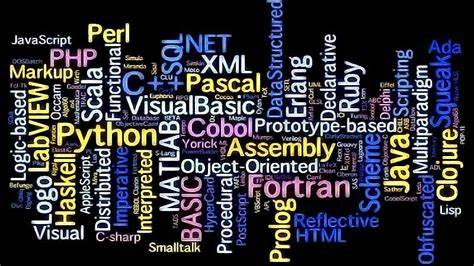
\includegraphics[width=1.\textwidth]{langs}
		\end{column}
		
		\begin{column}{.6\textwidth}
			
			\begin{block}{What is System programming language}
				A system programming language is a programming language used for system programming; such languages are designed for writing system software, which usually requires different development approaches when compared with application software. Edsger Dijkstra refers to these language as Machine Oriented High Order Languages.  [wikipedia]
			\end{block} 
			
			
			\begin{itemize}
				\item General-purpose programming languages (Java, Pascal, etc.) tend to focus on generic features. This generic quality typically comes at the cost of denying direct access to the machine's internal workings, and this often has negative effects on performance.
				
			\end{itemize}
			
			
		\end{column}
		
		
	\end{columns}
	
	
\end{frame}




%-------------------------------------------------
\begin{frame}[plain]
	\frametitle{Introduction}
	
	
	
	\begin{columns}
		
		\begin{column}{.4\textwidth}
			
			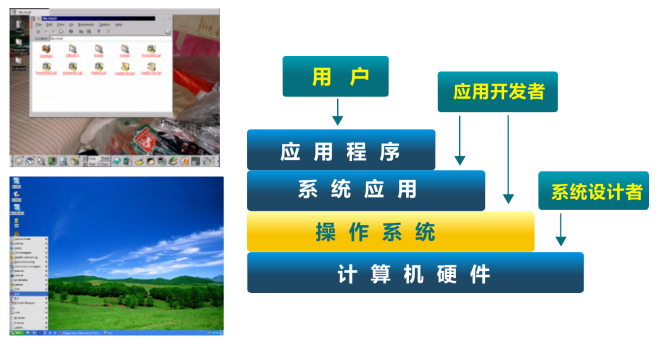
\includegraphics[width=1.\textwidth]{os-position}
			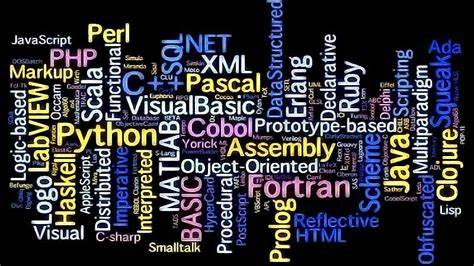
\includegraphics[width=1.\textwidth]{langs}
		\end{column}
		
		\begin{column}{.6\textwidth}
			
			\begin{block}{What is System programming language}
				A system programming language is a programming language used for system programming; such languages are designed for writing system software, which usually requires different development approaches when compared with application software.   [wikipedia]
			\end{block} 
			
			
			\begin{itemize}
				\item System languages are for performance and ease of access to the underlying hardware while still providing high-level programming concepts like structured programming. Examples include  Executive Systems Problem Oriented Language (ESPOL), which is similar to ALGOL in syntax but tuned to their respective platforms. 
				
			\end{itemize}
			
			
		\end{column}
		
		
	\end{columns}
	
	
\end{frame}


%-------------------------------------------------
\begin{frame}[plain]
	\frametitle{Introduction}
	
	
	
	\begin{columns}
		
		\begin{column}{.4\textwidth}
			
			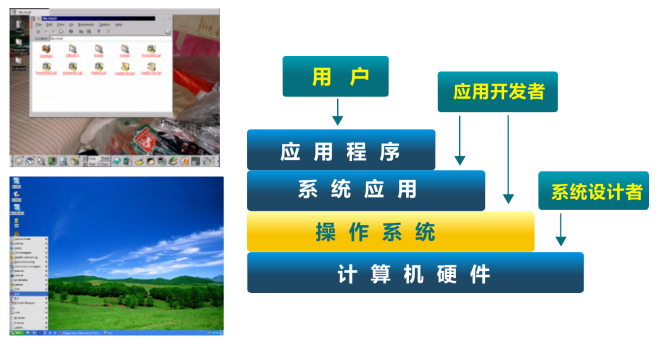
\includegraphics[width=1.\textwidth]{os-position}
			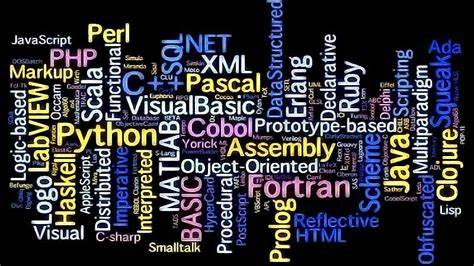
\includegraphics[width=1.\textwidth]{langs}
		\end{column}
		
		\begin{column}{.6\textwidth}
			
			\begin{block}{What is System programming language}
				A system programming language is a programming language used for system programming; such languages are designed for writing system software, which usually requires different development approaches when compared with application software.   [wikipedia]
			\end{block} 
			
			
			\begin{itemize}
				\item Some languages straddle the system and application domains, bridging the gap between these uses. The canonical example is C, which is used widely for both system and application programming. Some modern languages also do this such as Rust and Swift.
				
			\end{itemize}
			
			
		\end{column}
		
		
	\end{columns}
	
	
\end{frame}


%-------------------------------------------------
\begin{frame}[plain]
	\frametitle{Introduction}
	
	\centering
	Major System programming languages
	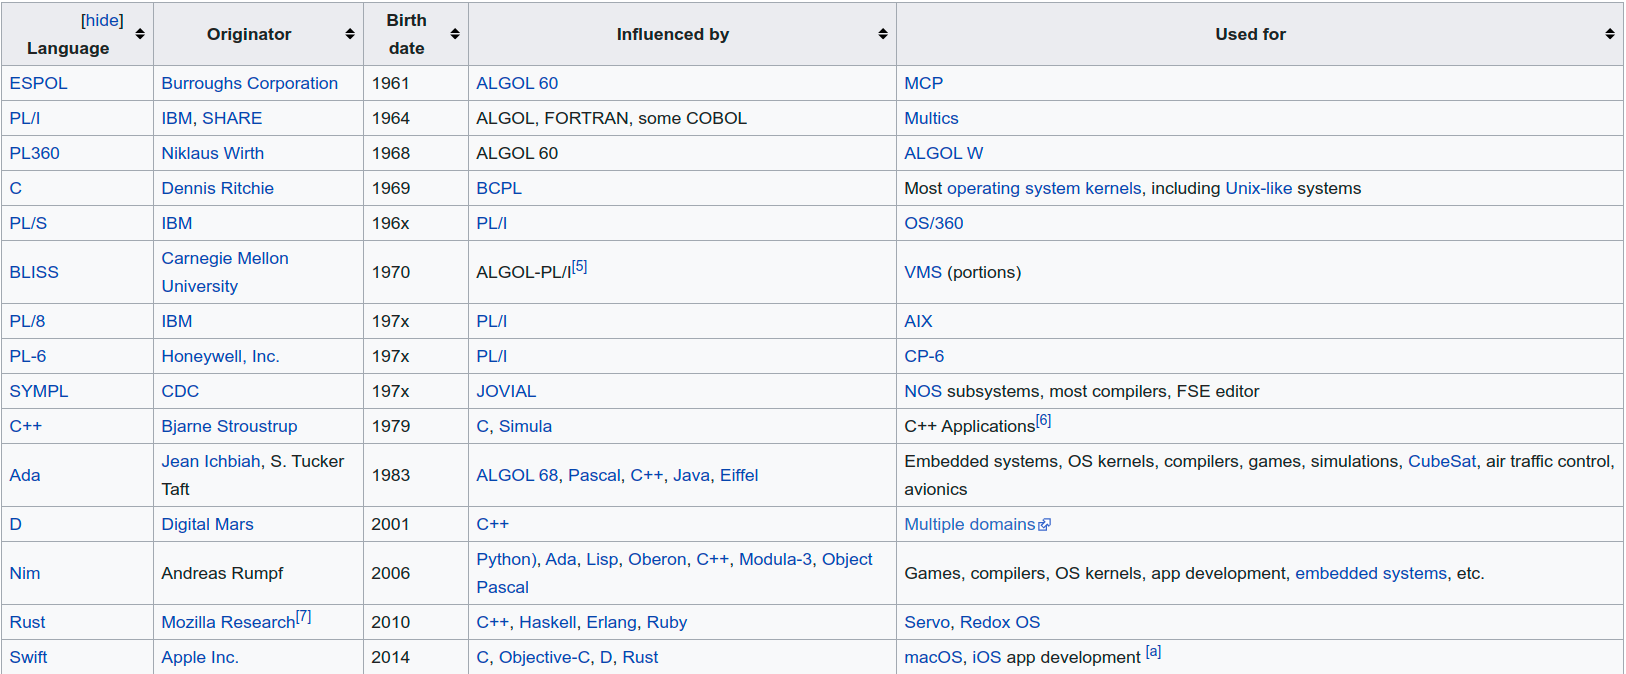
\includegraphics[width=1.\textwidth]{sys-langs}
\end{frame}
%-------------------------------------------------

%-------------------------------------------------
\begin{frame}[plain]
	\frametitle{Introduction}
	
	\centering
	Some OS based on Non-C language
	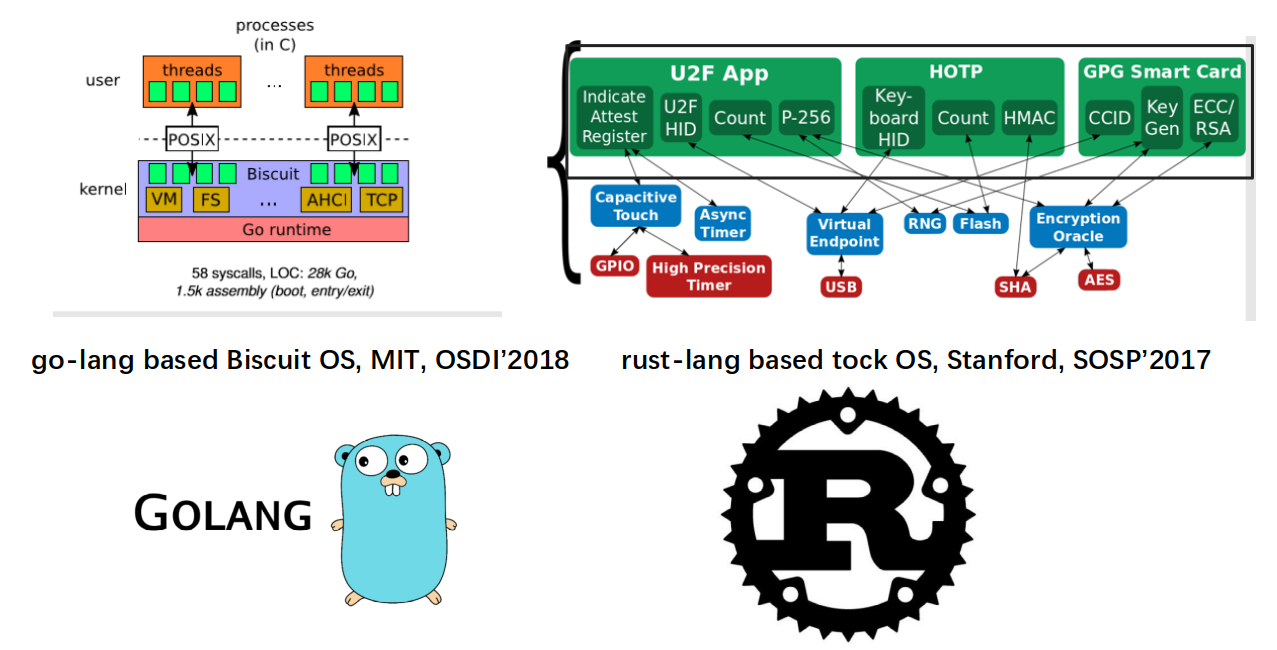
\includegraphics[width=.9\textwidth]{biscuit-tock-os}
把\end{frame}


%-------------------------------------------------
\begin{frame}[plain]
	\frametitle{History -- MCP \& ESPOL}
	
	

\begin{columns}
	
	\begin{column}{.4\textwidth}
		\centering
		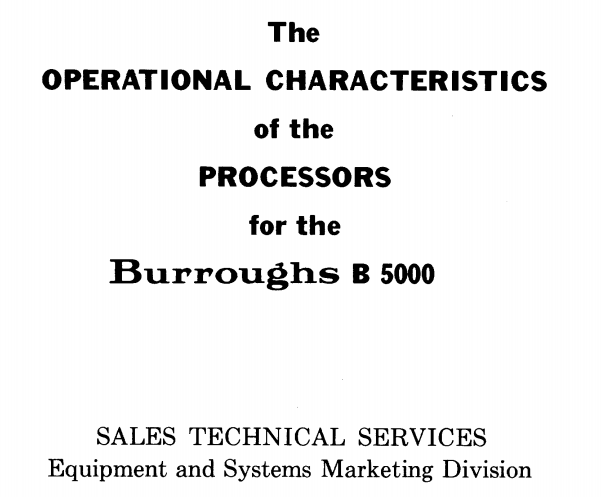
\includegraphics[width=.5\textwidth]{b5k}
		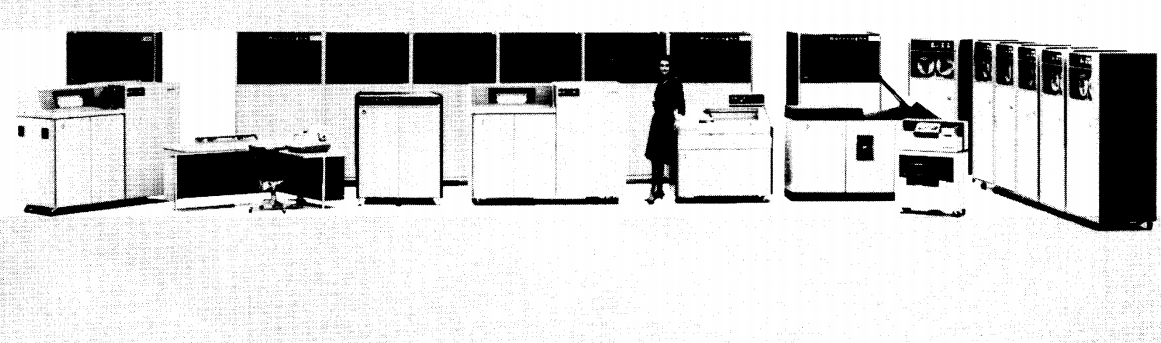
\includegraphics[width=1.\textwidth]{b5k-machine}
		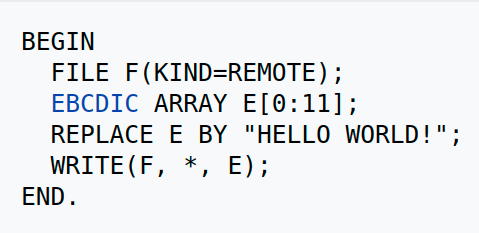
\includegraphics[width=.8\textwidth]{helloworld-algol60}
	\end{column}
	
	\begin{column}{.6\textwidth}
		
		
		\begin{itemize}
			\item The MCP (Master Control Program), the first OS written exclusively in a high-level language (HLL), is the proprietary operating system of the Burroughs small, medium and large systems.
			\item MCP provides virtual memory, file system with hierarchical directory structures, processes are called "Jobs" and "Tasks.", software components and libraries.
			
			\item  Originally written in 1961 in ESPOL (Executive Systems Programming Language), which itself was an extension of Burroughs Extended ALGOL,
		\end{itemize}
		
		
	\end{column}
	
	
\end{columns}

\end{frame}






%-------------------------------------------------
\begin{frame}[plain]
	\frametitle{History -- MCP \& ESPOL}
	
	ESPOL (Executive Systems Programming Language), extension of Burroughs Extended ALGOL.
	\centering
	%			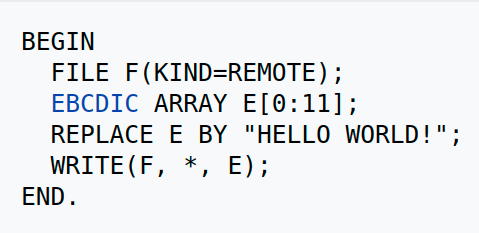
\includegraphics[width=.3\textwidth]{helloworld-algol60}
	
	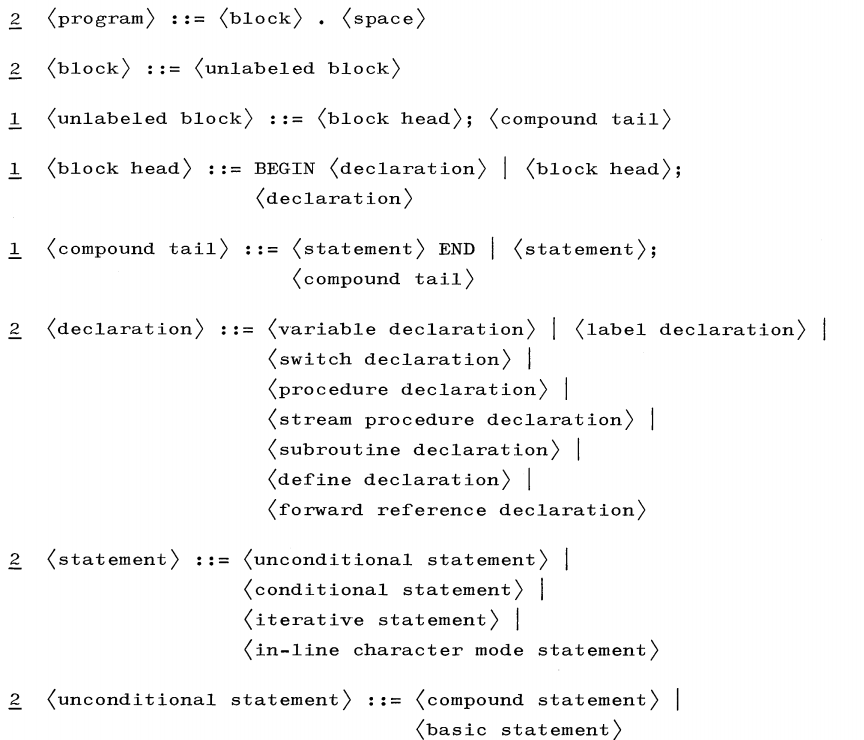
\includegraphics[width=.5\textwidth]{espol-syntax}
	
\end{frame}

%-------------------------------------------------
\begin{frame}[plain]
	\frametitle{History -- MULTICS \& PL/I}
	
	MULTICS OS \& PL/I language
	
    \begin{itemize}
		\item Multics (Multiplexed Information and Computing Service) is an influential early time-sharing operating system. Virtually all modern operating systems were heavily influenced by Multics – often through Unix.
		
		\item PL/I (Programming Language One, and sometimes written PL/1)is a procedural, imperative computer programming language developed by IBM.
	\end{itemize}
	\centering

	
	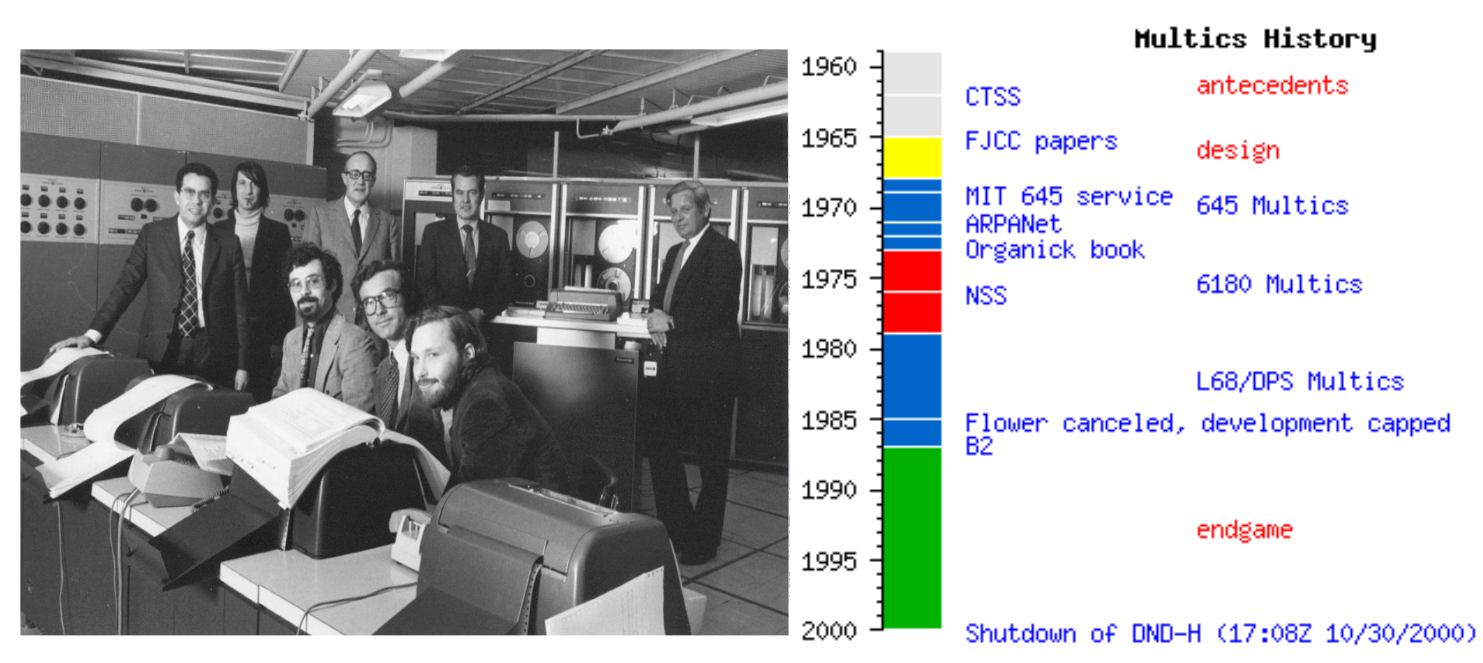
\includegraphics[width=.7\textwidth]{multics-history}
	
%	MIT: Prior pioneering work
%	Bell Labs: Engineering, Business management, Communications
%	General Electric: Hardware
	
	
	
\end{frame}


%-------------------------------------------------
\begin{frame}[plain]
	\frametitle{History -- MULTICS \& PL/I}
	
	Development on (heavily loaded) CTSS or MULTICS
	
	
	\begin{itemize}
		\item MIT: Prior pioneering work
		\item Bell Labs: Engineering, Business management, Communications
		\item General Electric: Hardware
	\end{itemize}
	\centering
	
	
	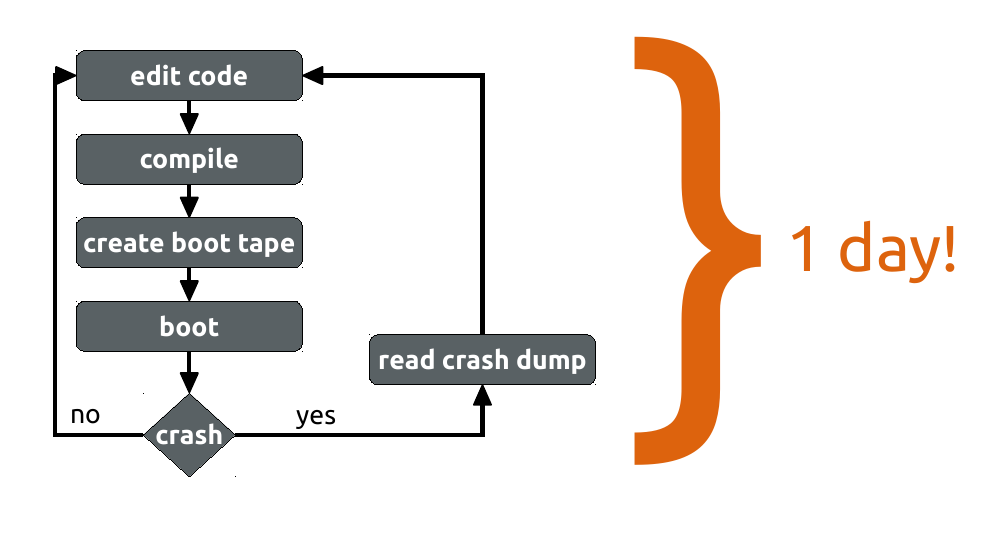
\includegraphics[width=.7\textwidth]{devel-ctss}
	
	%	MIT: Prior pioneering work
	%	Bell Labs: Engineering, Business management, Communications
	%	General Electric: Hardware
	
	
	
\end{frame}

%-------------------------------------------------
\begin{frame}[plain]
	\frametitle{History -- MULTICS \& PL/I}
	
	The Choice of PL/I
    \begin{itemize}
%		\item The big two languages in the US at the time were of course FORTRAN and COBOL.
		\item PL/I (Programming Language One, and sometimes written PL/1)is a procedural, imperative computer programming language developed by IBM.
		\item In 1964, when Project MAC at MIT sought to build a successor
		to their Compatible Time-sharing System (CTSS), they selected
		the language (PL/I) before writing any code.
		\item The decision to use PL/I in Multics was seen by its creators as a
		great strength. But that the compiler was unavailable for so long (and when
		was available, performed poorly) was a nearly-fatal weakness.
		\item The dynamic linking and paging facilities of the Multics environment have the effect of making available in virtual storage only those specific pages of those particular procedures which are referenced during an execution of the compiler. 
		
	
	\end{itemize}
%	\centering
	
	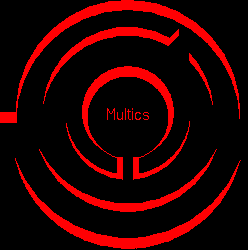
\includegraphics[width=.1\textwidth]{multics-logo}
	\tiny Multics Logo \\ https://multicians.org/pl1.html \\ https://multicians.org/pl1-raf.html \\ http://teampli.net/plisprg.html
	
	
\end{frame}

%-------------------------------------------------
\begin{frame}[plain]
	\frametitle{History -- NUIX \& C}
	
	The birth of Unix
	\begin{itemize}

		\item Bell Labs pulled out of the Multics project in 1969.
		
		\item A researcher formerly on the Multics effort, Ken Thompson,
		implemented a new operating system(was implemented entirely in assembly) for the PDP-7.
		\item The system was later ported to the PDP-11/20, where it was
		named Unix — a play on “eunuchs” and a contrast to the top-
		down complexity of Multics. 
		
		
		
	\end{itemize}
	
	
\end{frame}


%-------------------------------------------------
\begin{frame}[plain]
	\frametitle{History --Unix \& high-level languages}
	
	B --> C
	\begin{itemize}
		
		\item The interpreted language B (a BCPL derivative), was present in
		Unix, but only used for auxiliary functionality, e.g. the assembler.
		
		\item Some of the B that was in use in Unix was replaced with
		assembly for reasons of performance.
		\item Dennis Ritchie and Thompson developed a B-inspired language
		focused on better abstracting the machine, naming it “C”. 
		\item Perhaps contrary to myth, C and Unix were not born at the
		same instant — they are siblings, not twins!
		
		
	\end{itemize}
	
	
\end{frame}


%-------------------------------------------------
\begin{frame}[plain]
	\frametitle{History --Unix \& high-level languages}
	
	The C revolution
	\begin{itemize}
		
		\item C is rightfully called “portable assembly”: it is designed to
		closely match the abstraction of the machine itself.
		
		\item C features memory addressability at its core.
		\item Unlike PL/I, C grew as concrete needs arose. 
		\item e.g., C organically adopted important facilities like macro
		processing through the C preprocessor.
		\item  Standardization efforts came late and were contentious: C
		remains infamous for its undefined behaviors.
		
		
	\end{itemize}
	
	
\end{frame}


%-------------------------------------------------
\begin{frame}[plain]
	\frametitle{History --Unix \& high-level languages}
	
	Operating systems in the 1980s
	
	\begin{itemize}
		
		\item  As the minimal abstraction above the machine, C — despite its
		blemishes — proved to be an excellent fit for operating systems
		implementation
		
		\item With few exceptions, operating systems — Unix or otherwise —
		were implemented in C throughout the 1980s
		
		\item  Other systems existed as research systems, but struggled to
		offer comparable performance to C-based systems
		
		
		
	\end{itemize}
	
	
\end{frame}


%-------------------------------------------------
\begin{frame}[plain]
	\frametitle{History --Unix \& high-level languages}
	
	Operating systems in the 1990s
	
	\begin{itemize}
		
		\item   In the 1990s, object oriented programming came into vogue,
		with languages like C++ and Java
		
		\item By the mid-1990s, C-based systems were thought to be relics
		
		\item ...but the systems putatively replacing them were rewrites —
		and suffered from rampant Second System Syndrome
		
		\item They were infamously late (e.g. Apple’s Copland), infamously
		slow (e.g. Sun’s Spring), or both (Taligent’s Pink)
		
		\item Java-based operating systems like Sun’s JavaOS fared no
		better; hard to interact with hardware without unsigned types.
		
	\end{itemize}
	
	
\end{frame}


%-------------------------------------------------
\begin{frame}[plain]
	\frametitle{History --Unix \& high-level languages}
	
	Operating systems in the 2000s
	
	\begin{itemize}
		
		\item   With the arrival of Linux, Unix enjoyed a resurgence, and
		C-based operating systems became deeply entrenched
		
		
		\item With only a few exceptions (e.g., Haiku), serious attempts at
		C++-based kernels withered
		
		
		\item At the same time, non\-Java/non-C++ languages blossomed:
		first Ruby, and then Python and JavaScript
		
		
		\item These languages were focused on ease of development rather
		than performance and there appears to be no serious effort
		to implement an operating system in any of these
		
		
	\end{itemize}
	
\end{frame}
%-------------------------------------------------
\begin{frame}[plain]
	\frametitle{History --Unix \& high-level languages}
	
	Systems software  in the 2010s
	
	\begin{itemize}
		
		\item  Systems programmers began pining for something different: the
		performance of C, but with more powerful constructs as enjoyed
		in other languages
		
		\item High-performance JavaScript runtimes allowed for a surprising
		use in node.js — but otherwise left much to be desired
		
		\item Bell Labs refugees at Google developed Go, which solves some
		problems, but with many idiosyncrasies
		
		\item  Go, JavaScript and others are garbage collected, making
		interacting with C either impossible or excruciatingly slow
		
		\item Rust is a systems software programming language designed
		around safety, parallelism, and speed
		
		
	\end{itemize}
	
\end{frame}

%-------------------------------------------------
\begin{frame}[plain]
	\frametitle{History --Unix \& high-level languages}
	
	Rust \&OS in the 2010s
	
	\begin{itemize}
		
		\item  First attempt at an operating system kernel in Rust seems to be
		Alex Light’s Reenix, ca. 2015: a re-implementation of a teaching
		operating system in Rust as an undergrad thesis
		
		
		\item  Since Reenix’s first efforts, there have been quite a few small
		systems in Rust, e.g.: Redox, Tifflin, Tock, intermezzOS,
		RustOS/QuiltOS, Rux, and Philipp Oppermann’s Blog OS, and rcore.
		
		\item Some of these are teaching systems (intermezzOS, Blog OS),
		some are unikernels (QuiltOS) and/or targeted at IoT (Tock)
		
		
	\end{itemize}
	\LARGE
	C based OS will dominate the development of OS?  \\
	Rust based OS will be the future?
\end{frame}
%-------------------------------------------------

%-------------------------------------------------
\begin{frame}[plain]
	\frametitle{References}

	\begin{itemize}
		
		\item Is it time to rewrite the operating system in Rust? Bryan Cantrill, tech talk, 2018
		
		
		
		
	\end{itemize}
	
	
\end{frame}
%-------------------------------------------------
%-------------------------------------------------
\end{document}